\documentclass[parskip=full]{scrartcl}
\usepackage[top=2.5cm, bottom=2.5cm, left=2.5cm, right=2.5cm]{geometry}
\usepackage[utf8]{inputenc}
\usepackage[T1]{fontenc}
\usepackage[german]{babel}
\usepackage[pangram]{blindtext}
\usepackage{hyperref}
\usepackage{graphicx}

\hypersetup{
  colorlinks=false,
  linktoc=all,
  hidelinks,
}

\title{Pflichtenheft}
\subtitle{Implementierung eines OPC UA Systemadapters für den Industrial Data Space}
\author{
    M. Armbruster\\
    D. Kahles\\
    H. Lehmann\\
    M. Schwarzmann\\
    N. Wilhelm
}
\begin{document}
\maketitle
\tableofcontents
\pagebreak

\section{Einleitung}
\Blindtext[1]

\section{Zielbestimmung}
Der Systemadapter dient dem Ziel, die Funktion von OPC UA zu demonstrieren, ohne eine konkrete Produktionsanlage
benutzen zu müssen. Somit kann beim Kunden das Protokoll flexibler vorgestellt werden. Hierzu soll das Programm
sowohl eine Produktionsanlage simulieren und den Status grafisch darstellen, als auch auch eine Überwachungskonsole
bereitstellen, die über OPC UA Werte der Anlage abfragt.\\
\begin{center}
    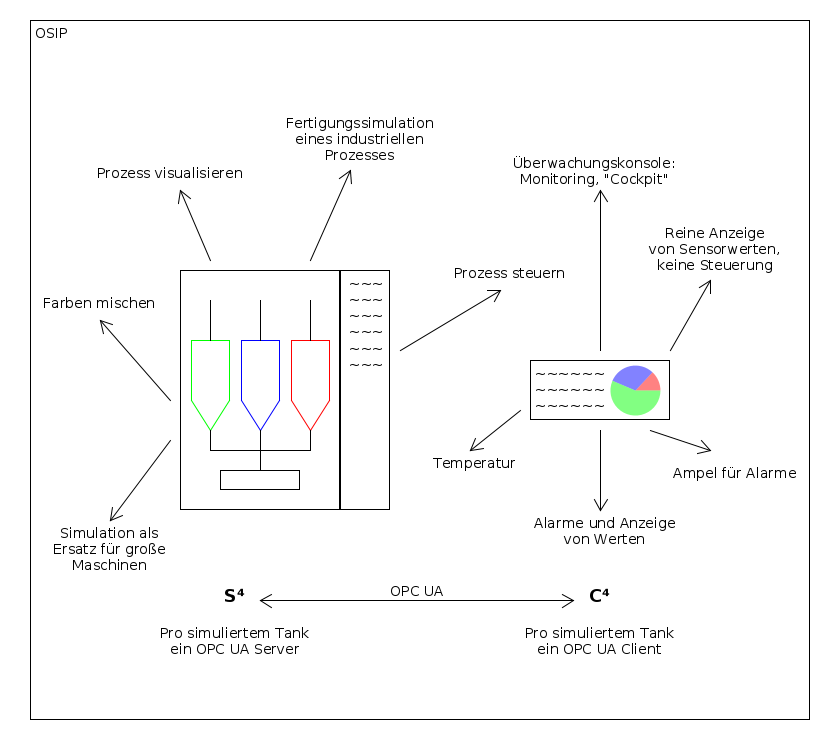
\includegraphics[scale=0.5]{../system-sketch.png}
\end{center}

\newpage
\section{Produkteinsatz}
\subsection{Anwendungsbereiche}
Das Produkt wird verwendet, um OPC UA und dessen Möglichkeiten zu präsentieren.
Insbesondere soll es einfacher aufzubauen und zu zeigen sein als reale Fertigungssimulationen.
Dies kann zum Beispiel auf Messen oder direkt bei potenziellen Kunden geschehen.
\subsection{Zielgruppen}
Die Zielgruppe umfasst Personen, die sich mit OPC UA auskennen und es potenziellen Anwendern vorführen möchten.
Dazu zählen insbesondere Mitglieder der OPC Fundation, die die Verbreitung des Protokolls fördern wollen,
aber auch Softwareentwickler die OPC UA konforme Software herstellen und möglichen Kunden auf einfache Art und
Weise die Funktionalität von OPC UA präsentieren wollen.
Die potenziellen Anwender haben meist keine Erfahrung mit OPC UA, sind aber für Industrieanlagen verantwortlich
die von OPC UA profitieren würden.

\subsection{Betriebsbedingungen}
Das Produkt kann entweder auf Messen, in Büros oder in Fertigungshallen direkt bei Kunden verwendet werden,
so lange die eingesetzte Hardware (siehe \ref{Hardware}) keine Probleme mit den Umgebungsbedingungen hat.

\section{Produktumgebung}
\subsection{Software}
Das Produkt erfordert einen Computer, auf dem das Betriebssystem Microsoft Windows 7, 8.1 oder 10 installiert ist,
oder auf dem Canonical Ubuntu 14.04 oder 16.04 installiert ist. Außerdem ist das Oracle Java Runtime Environment in Version 1.8
notwendig. Wenn die Fertigungssimulation und die Überwachungskonsole auf unterschiedlichen Computern laufen,
ist eine TCP/IP Verbindung mit einer Bandbreite von 100 MBit/s und einer Latenz von maximal 100 ms zwischen den Computern notwendig.
Außerdem wird eventuell (siehe \ref{fertigung-optional} und \ref{konsole-optional}) unter Ubuntu 16.04 die Containersoftware Docker
ab Version 1.10.3 unterstützt, mit dem die beiden Softwareteile isoliert in Containern verteilt und ausgeführt werden können.

\subsection{Hardware}
\label{Hardware}
Es ist ein Laptop oder Desktopcomputer notwendig, der eines der oben genannten Betriebssysteme unterstützt.
Zudem sind mindestens 2GB Arbeitsspeicher notwendig. Die CPU muss die x86 Architektur unterstützen, zwei Kerne haben und mit
mindestens 2GHz getaktet sein.

\section{Funktionale Anforderungen}
\subsection{Fertigungssimulation}
\subsubsection{Funktionalität}
\begin{enumerate}
\item[FA10] Die Zu- und Abflussmengen der oberen Flüssigkeitstanks können seperat eingestellt werden.
\item[FA20] Die Abflussmenge des unteren Flüssigkeitstanks kann eingestellt werden. Die Zuflussmenge ergibt sich aus der Summe der Abflussmengen der oberen Tanks.
\item[FA30] Der untere Tank enthält einen motorbetriebenen Mischer, dessen Drehzahl eingestellt werden kann. Dabei kann die Drehzahl in einem Bereich zwischen
0 und 300 Umdrehungen pro Minute gewählt werden.
\item[FA40] Jedem der oberen Tanks ist eine Flüssigkeitsfarbe zugeordnet. Die Farbe des unteren Tanks ergibt sich aus dem Mischungsverhältnis der oberen Tanks. Dabei wird
angenommen, dass die Flüssigkeiten der oberen Tanks die selbe Deckkraft haben.
\item[FA50] Es gibt eine .jar Datei, die bei Ausführung die Fertigungssimulation startet.
\end{enumerate}

\subsubsection{GUI Darstellung}
\begin{enumerate}
\item[FA110] Der Mischer im unteren Flüssigkeitstank wird durch ein sich drehendes GUI Element dargestellt.
Die Umdrehungsgeschwindigkeit repräsentiert die Drehzahl des Mischermotors.
\item[FA120] Der Füllstand der Flüssigkeitstanks wird durch das Füllen der Tanks in der Farbe ihrer Flüssigkeit dargestellt.
\item[FA130] Die einstellbaren Parameter können in einem Unterfenster eingestellt werden. Darin existiert für jeden Tank ein eigener Reiter, der die 
tankspziefischen Einstellungen wie zum Beispiel Zu- und Abflussmengen, Zuflusstemperaturen oder Motordrehzahlen (siehe FA10 bis FA30) enthält.
Diese Parameter werden durch Schieberegler eingestellt.
\end{enumerate}

\subsubsection{Optionale Funktionalität}
\label{fertigung-optional}
\begin{enumerate}
\item[FA240] Es gibt ein Dockerimage zur einfachen Verteilung und isolierten Ausführung der Fertigungssimulation
\end{enumerate}

\subsection{Überwachungskonsole}
\subsubsection{Funktionalität}
\begin{enumerate}
\item[310] Die Überwachungskonsole zeigt die Farbe der Flüssigkeitstanks an.
\item[320] Die Überwachungskonsole zeigt die Zu-, und Abflussmenge der oberen Flüssigkeitstanks an.
\item[330] Die Überwachungskonsole zeigt die Abflussmenge des unteren Flüssigkeitstanks an.
\item[340] Die Überwachungskonsole zeigt die Drehzahl des Mischermontors an.
\item[350] Alle angezeigte Sensordaten werden mit der eingestellten Aktualisierungsfrequenz aktualisiert.
\item[360] Der Benutzer kann die Anzeige der Füllstands- und Temperaturverläufe für jeden Tank ein- und ausschalten.
\item[370] Es gibt eine .jar Datei, die bei Ausführung die Überwachungskonsole startet.
\end{enumerate}
\subsubsection{GUI Darstellung}
\begin{enumerate}
\item[410] Die Überwachungskonsole enthält für die Einstellungen ein getrenntes Fenster.
\item[420] Das Einstellungsfenster hat zwei Reiter: ``Allgemeines'' und ``Empfangene Daten''.
\item[430] Im Reiter ``Allgemeines'' kann die Aktualisierungsfrequenz im Bereich zwischen 20 und 4000 Millisekunden gewählt werden.
\item[440] Im Reiter ``Empfangene Daten'' kann für jeden Tank die Anzeige des Füllstands und Temperaturverläufe mittels Checkboxen ein- und ausgeschaltet werden.
\end{enumerate}

\subsubsection{Optionale Funktionalität}
\label{konsole-optional}
\begin{enumerate}
\item[FA540] Es gibt ein Dockerimage zur einfachen Verteilung und isolierten Ausführung der Überwachungskonsole
\end{enumerate}

\section{Nichtfunktionale Anforderungen}
\Blindtext[1]

\section{Produktdaten}
\Blindtext[1]

\section{Globale Testfälle}
\Blindtext[1]

\section{Systemmodelle}
\subsection{Szenarien}
\subsubsection{Szenario 2: Konfigurierbarkeit}
Als Philipp zu ihm kommt, will Manuel ihm die Funktion von OPC UA demonstrieren.
Als erstes ändert er in der Fertigungssimulation den Zu- und Abfluss bei zwei der Tanks. Nun sehen die beiden, wie
sich die von der Überwachungskonsole angezeigten Werte für Zu- und Abfluss mit der nächsten Aktualisierung ändern. Die
Farbe im Zielcontainer ändert sich langsam, während sich das Mischungsverhältnis der Flüssigkeiten ändert. Auch diese
Werte werden in der Überwachungskonsole jeweils aktualisiert.

Als nächstes navigiert Manuel in das Einstellungsmenü seines Clients. Dort geht er in den Punkt ``Empfangene Daten'' und
wählt zusätzlich zu den bisher angezeigten Werten noch die Kategorien ``Füllstand'' und ``Motordrehzahl'' beim unteren Tank
an. Nach einem Klick auf ``Übernehmen'' sehen die beiden, wie in der Überwachungskonsole neue Anzeigen aufgetaucht sind,
die die neuen Werte darstellen. Außerdem entsteht ein neuer Reiter bei der Überwachungsanzeige des unteren Tanks,
in dem Philipp den Füllstandsverlauf ansehen kann.

Philipp merkt nun an, dass ihm die Flexibilität der empfangenen Daten sehr gefällt. Das Aktualisierungsintervall von
einer Sekunde sei aber in manchen der Fertigungsprozesse zu lang, da in manchen kritischen Zuständen sehr schnell
automatisch reagiert werden muss, etwa wenn Schwellenwerte überschritten werden. Daraufhin ändert Manuel in den
Einstellungen das Aktualisierungsintervall von 1000ms auf 250ms. Anschließend sehen beide, wie sich die Werte in der
Überwachungskonsole tatsächlich vier Mal pro Sekunde aktualisieren.

\subsubsection{Szenario 3: Alarme}
Philipp ist zunehmend an OPC UA interessiert, hat aber noch letzte Zweifel. Er merkt an, dass die Abfrage der Daten
zwar gut funktioniert, eine wirkliche \"Uberwachung aber noch einen Wrapper f\"ur das Programm ben\"otigen w\"urde,
um ungew\"ohnliche Zust\"ande in der Fertigung automatisch zu bemerken und darauf aufmerksam zu machen.
Manuel merkt an, dass das ein guter Einwand ist und dass OPC UA auch daf\"ur eine passende Funktionalit\"at besitzt.

Er \"offnet das Einstellungsmen\"u der \"Uberwachungskonsole und erstellt einen neuen Alarm. Um die Flexibilit\"at
von OPC UA erneut zu demonstrieren fragt er Philipp, welchen Zustand er gerne abfangen w\"urde. Philipp w\"urde gerne
abfangen, wenn ein Tank \"uberzulaufen droht. Er schl\"agt daf\"ur als Grenze einen F\"ullstand von 95\% vor.
Manuel gibt also in der \"Uberwachungskonsole 95\% als Grenze an und w\"ahlt einen Tank, f\"ur den der Alarm stattfinden soll.
Dann speichert er die neuen Einstellungen.

Anschlie{\ss}end dreht er in der Fertigungssimulation den Zufluss des entsprechenden Tanks auf, woraufhin der F\"ullstand
zu steigen beginnt. In der Fertigungssimulation ist der Steigende F\"ullstand zu sehen, in der \"Uberwachungskonsole werden
steigende Werte angezeigt.
Darauf wird der F\"ullstand von 95\% erreicht und in der \"Uberwachungskonsole der Alarm ausgel\"ost. Manuel
beschlie{\ss}t, nicht zu handeln und der Tank l\"auft \"uber. Danach w\"ahlt Philipp in den Einstellungen der
Fertigungssimulation die Option ``zur\"ucksetzen'' woraufhin wieder die Standardkonfiguration angezeigt wird.

\subsection{Anwendungsfälle}
\Blindtext[1]

\subsection{Dynamische Modelle}
\Blindtext[1]

\subsection{Statische Modelle}
\Blindtext[1]

\section{Nutzerinterface-Skizzen}
\Blindtext[1]

\section{Glossar}
\Blindtext[1]

\end{document}
